\documentclass[
  bibliography=totoc,     % Literatur im Inhaltsverzeichnis
  captions=tableheading,  % Tabellenüberschriften
  titlepage=firstiscover, % Titelseite ist Deckblatt
]{scrartcl}

% Paket float verbessern
\usepackage{scrhack}

% Warnung, falls nochmal kompiliert werden muss
\usepackage[aux]{rerunfilecheck}

% unverzichtbare Mathe-Befehle
\usepackage{amsmath}
% viele Mathe-Symbole
\usepackage{amssymb}
% Erweiterungen für amsmath
\usepackage{mathtools}

% Fonteinstellungen
\usepackage{fontspec}
% Latin Modern Fonts werden automatisch geladen
% Alternativ zum Beispiel:
%\setromanfont{Libertinus Serif}
%\setsansfont{Libertinus Sans}
%\setmonofont{Libertinus Mono}

% Wenn man andere Schriftarten gesetzt hat,
% sollte man das Seiten-Layout neu berechnen lassen
\recalctypearea{}

% deutsche Spracheinstellungen
\usepackage[ngerman]{babel}


\usepackage[
  math-style=ISO,    % ┐
  bold-style=ISO,    % │
  sans-style=italic, % │ ISO-Standard folgen
  nabla=upright,     % │
  partial=upright,   % │
  mathrm=sym,        % ┘
  warnings-off={           % ┐
    mathtools-colon,       % │ unnötige Warnungen ausschalten
    mathtools-overbracket, % │
  },                       % ┘
]{unicode-math}

% traditionelle Fonts für Mathematik
\setmathfont{Latin Modern Math}
% Alternativ zum Beispiel:
%\setmathfont{Libertinus Math}

\setmathfont{XITS Math}[range={scr, bfscr}]
\setmathfont{XITS Math}[range={cal, bfcal}, StylisticSet=1]

% Zahlen und Einheiten
\usepackage[
  locale=DE,                   % deutsche Einstellungen
  separate-uncertainty=true,   % immer Unsicherheit mit \pm
  per-mode=symbol-or-fraction, % / in inline math, fraction in display math
]{siunitx}

% chemische Formeln
\usepackage[
  version=4,
  math-greek=default, % ┐ mit unicode-math zusammenarbeiten
  text-greek=default, % ┘
]{mhchem}

% richtige Anführungszeichen
\usepackage[autostyle]{csquotes}

% schöne Brüche im Text
\usepackage{xfrac}

% Standardplatzierung für Floats einstellen
\usepackage{float}
\floatplacement{figure}{htbp}
\floatplacement{table}{htbp}

% Floats innerhalb einer Section halten
\usepackage[
  section, % Floats innerhalb der Section halten
  below,   % unterhalb der Section aber auf der selben Seite ist ok
]{placeins}

% Seite drehen für breite Tabellen: landscape Umgebung
\usepackage{pdflscape}

% Captions schöner machen.
\usepackage[
  labelfont=bf,        % Tabelle x: Abbildung y: ist jetzt fett
  font=small,          % Schrift etwas kleiner als Dokument
  width=0.9\textwidth, % maximale Breite einer Caption schmaler
]{caption}
% subfigure, subtable, subref
\usepackage{subcaption}

% Grafiken können eingebunden werden
\usepackage{graphicx}

% schöne Tabellen
\usepackage{tabularray}
\UseTblrLibrary{booktabs, siunitx}

% Verbesserungen am Schriftbild
\usepackage{microtype}

% Literaturverzeichnis
\usepackage[
  backend=biber,
]{biblatex}
% Quellendatenbank
\addbibresource{lit.bib}
\addbibresource{programme.bib}

% Hyperlinks im Dokument
\usepackage[
  german,
  unicode,        % Unicode in PDF-Attributen erlauben
  pdfusetitle,    % Titel, Autoren und Datum als PDF-Attribute
  pdfcreator={},  % ┐ PDF-Attribute säubern
  pdfproducer={}, % ┘
]{hyperref}
% erweiterte Bookmarks im PDF
\usepackage{bookmark}

% Trennung von Wörtern mit Strichen
\usepackage[shortcuts]{extdash}

\author{%
  AUTOR A\\%
  \href{mailto:authorA@udo.edu}{authorA@udo.edu}%
  \and%
  AUTOR B\\%
  \href{mailto:authorB@udo.edu}{authorB@udo.edu}%
}
\publishers{TU Dortmund – Fakultät Physik}


\subject{V105}
\title{Das magnetische Moment}
\date{%
  Durchführung: 5.12.2023
  \hspace{3em}
  Abgabe: 11.12.2023
}

\begin{document}

\maketitle
\thispagestyle{empty}
\tableofcontents
\newpage

\section{Theorie}
\label{sec:Theorie}
\subsection{allgemeine Relaxationsgleichung und praktisches Beispiel des RC-Kreises}
Relaxation beschreibt die  Effekte welche beim Entfernen eines Systems aus seinem oszillierenden Zustands und seiner anschließenden Rückkehr (ohne Oszillation) in 
selbigen Zustand zustande kommen.Im allgemeinen gilt dabei 
\begin{equation}
    \frac{dA}{dt}=c[A(t)-A(\infty)]\,
\end{equation}
bzw. nach Integration und Auflösung nach A(t)
\begin{equation}
    A(t)=A(\infty) + [A(0)-A(\infty)]\cdot e^(ct)\,
\label{eqn:voreqn2}
\end{equation}



Ein praktisches Beispiel für einen Relaxationsvorgang stellen die Auf- und Entladung eines Kodensators im RC-Kreis dar. Aus dem Zusammenhang
\begin{equation}
     U_{C}= \frac{Q}{C}\,
    \label{eqn:eqn2}
\end{equation}
folgt mit dem Ohmschen Gesetz $I= \frac{U_{C}}{R}$ und der Ladungsänderung \begin{equation}
    dQ = Idt
    \label{eqn:eqn3}
\end{equation} 
das $ \frac{dQ}{dt} = (-)\frac{1}{RC}\cdot Q(t)$ gilt.
Mittels Integration folgt dann unter Berücksichtigung der Randbedingung $Q(\infty)=0$
\begin{equation}
Q(t)= Q(0)\cdot exp(-\frac{t}{RC})\,
\label{eqn:eq1}
\end{equation}
DIe Randbedingung folgt dabei aus der Tatsache das der Kondensator sich asymptotisch gegen 0 nähert für t gegen unendlich.
Für die Aufladefunktion des Kondensators bei Verbindung mit einer Spannungsquelle folgt mit ähnlichem Ansatz\\
$Q(t)=C U_{0}(1-exp(\frac{-t}{RC}))$\\
Die Größe RC wird als Zeitkonstante $\tau$ bezeichnet. Innerhalb eines dieser Zeitkonstanten ändert sich die Ladung um den Faktor $\frac{1}{e} \approx \qty{36.8}{\percent}$.
\subsection{Relaxations bei periodischer Auslenkung aus Gleichgewichtslage Anhand eines RC-Kreise}
In diesem Fall des RC-Kreise wird eine Äußere Spannung mit $U(t)=U_{0}\cdot cos(\omega t)$ betrachtet.
Für kleine Frequenzen $\omega$ ($\omega << \frac{1}{RC})$ ist die Kodensatorspannung $U_{c}$ gleich der äußeren Spannung $U_0$. Da der Auf- und Entladeprozess jedoch zeitlich 
durch die Zeitkonstante in seiner Dauer nicht beliebig schnell werden kann, ergibt sich bei steigender Frequenz ein Phasenunterschied zwischen $U_0$ und $U_C$. 
Da desweiteren die Äußere Spannung ein anderes Vorzeichen als die Kodensatorspannung hat, sinkt die Amplitude der Spannung am Kodensator.\\
Mathematisch kann dieses Problem folgender Weise betrachtet werden:\\
Als Grundansatz wählt man
\begin{equation}
    U_{C}(t)= A(\omega)cos(\omega t+ \varphi (\omega))  \,
    \label{eqn:ansatz}
\end{equation}
Mit dem zweiten Kirchhoffschen Gesetz ergibt sich
\begin{equation}
U_{0}cos(\omega t)= I(t)R + A(\omega)cos(\omega t+ \varphi (\omega)) \,
\label{eqn:eqn6}
\end{equation}
Aus \ref{eqn:eqn2} und \ref{eqn:eqn3} folgt dann 
\begin{equation}
I(t)= C\frac{dU_{C}}{dt}
\label{eqn:eqn7}
\end{equation}
Insgesamt ergibt sich dann durch einsetzen von \ref{eqn:eqn7} in \ref{eqn:eqn6}
\begin{equation}
    U_{0}cos(\omega t)= A \omega RC sin(\omega t + \varphi) + A(\omega)cos(\omega t+ \varphi (\omega)) \,
\label{eqn:eqn8}
\end{equation}
Aus der Gültigkeit dieser Gleichung lässt sich durch die Auswahl spezieller werte für t nach einigen Umformungen der Zusammenhang 
\begin{equation}
    \varphi (\omega) = arctan(-\omega RC)\,
    \label{eqn:phase1}
\end{equation}
für die Phasenverschiebung zwischen $U_{C}$ und $U_{0}$ herstellen.\\
Ebenfalls aus \ref{eqn:eqn8} folgt nach Umformung 
\begin{equation}
    A(\omega)= -\frac{sin(\varphi)}{\omega RC}\cdot U_{0}\,
    \label{eqn:amplitude1}
\end{equation}
oder durch verwendung von \ref{eqn:phase1}
\begin{equation}
    A(\omega)= \frac{U_{0}}{\sqrt{1+ (\omega RC)^2}}\,
    \label{eqn:amplitude2}
\end{equation}
als Zusammenhang zwischen der Amplitude von $U_{C}$.\\
Aus \ref{eqn:phase1} lässt sich erkenn, das die Phasendifferenz für kleine Frequenzen gegen 0 und für hohe Frequenzen gegen $\frac{\pi}{2}$ geht.\\
Für die Amplitude lässt sich aus \ref{eqn:amplitude2} leicht erkennen, dass $A$ für kleine Frequenzen gegen $U_{0}$ und für große Frequenzen gegen 0 geht.


\label{sec:Theorie}



\subsection{Integrationsverhalten des RC-Kreises}
Ein RC-Kreis, oder Tiefpass, kann als integrator dienen, wenn die Bedingung $\omega >> \frac{1}{RC}$ erfüllt ist. Es kann die proportionalität von $U_c$ zu $\int U(t) dt$ gezeit werden.
\begin{equation}
    U(t) = U_{R}(t) + U_C(t) = I(t) \cdot R + U_c(t)
    \label{eq:e9} %ZAHL MUSS NOCH ANGEPASST WERDEN
\end{equation}

Mit \ref{eqn:eqn7} wird I(t) ersetzt:\\

\begin{equation}
    U(t) = RC\frac{dU_C}{dt}
    \label{eq:e10} %ZAHL MUSS NOCH ANGEPASST WERDEN
\end{equation}

Wegen der Bedingung $\omega >> \frac{1}{RC}$ folgt dann:
\begin{equation}
    U_C(t) = \frac{1}{RC}\int_{0}^{t}U(t') dt'
    \label{eq:e11} %ZAHL MUSS NOCH ANGEPASST WERDEN
\end{equation}



 Theorie entnommen aus \cite{V353}

\section{Durchführung}
\label{sec:Durchführung}
\subsection{Aufbau}
Im Versuch ist ein Spannungsgenerator gegeben, der für die erste Messreihe nur über einen Tiefpass mit einem Oszilloskop verbunden ist, zu sehen in Abbildung \ref{foto1} 
Für die Aufnahme der zweiten Messreihe und zur messung zur Bestätigung der Integratorfunktion wird auch noch eine direkte Verbindung zwischen dem Spannungsgenerator und dem Oszilloskop eingeführt, zu sehen in Abbildung \ref{foto2}.
\begin{figure}
\centering
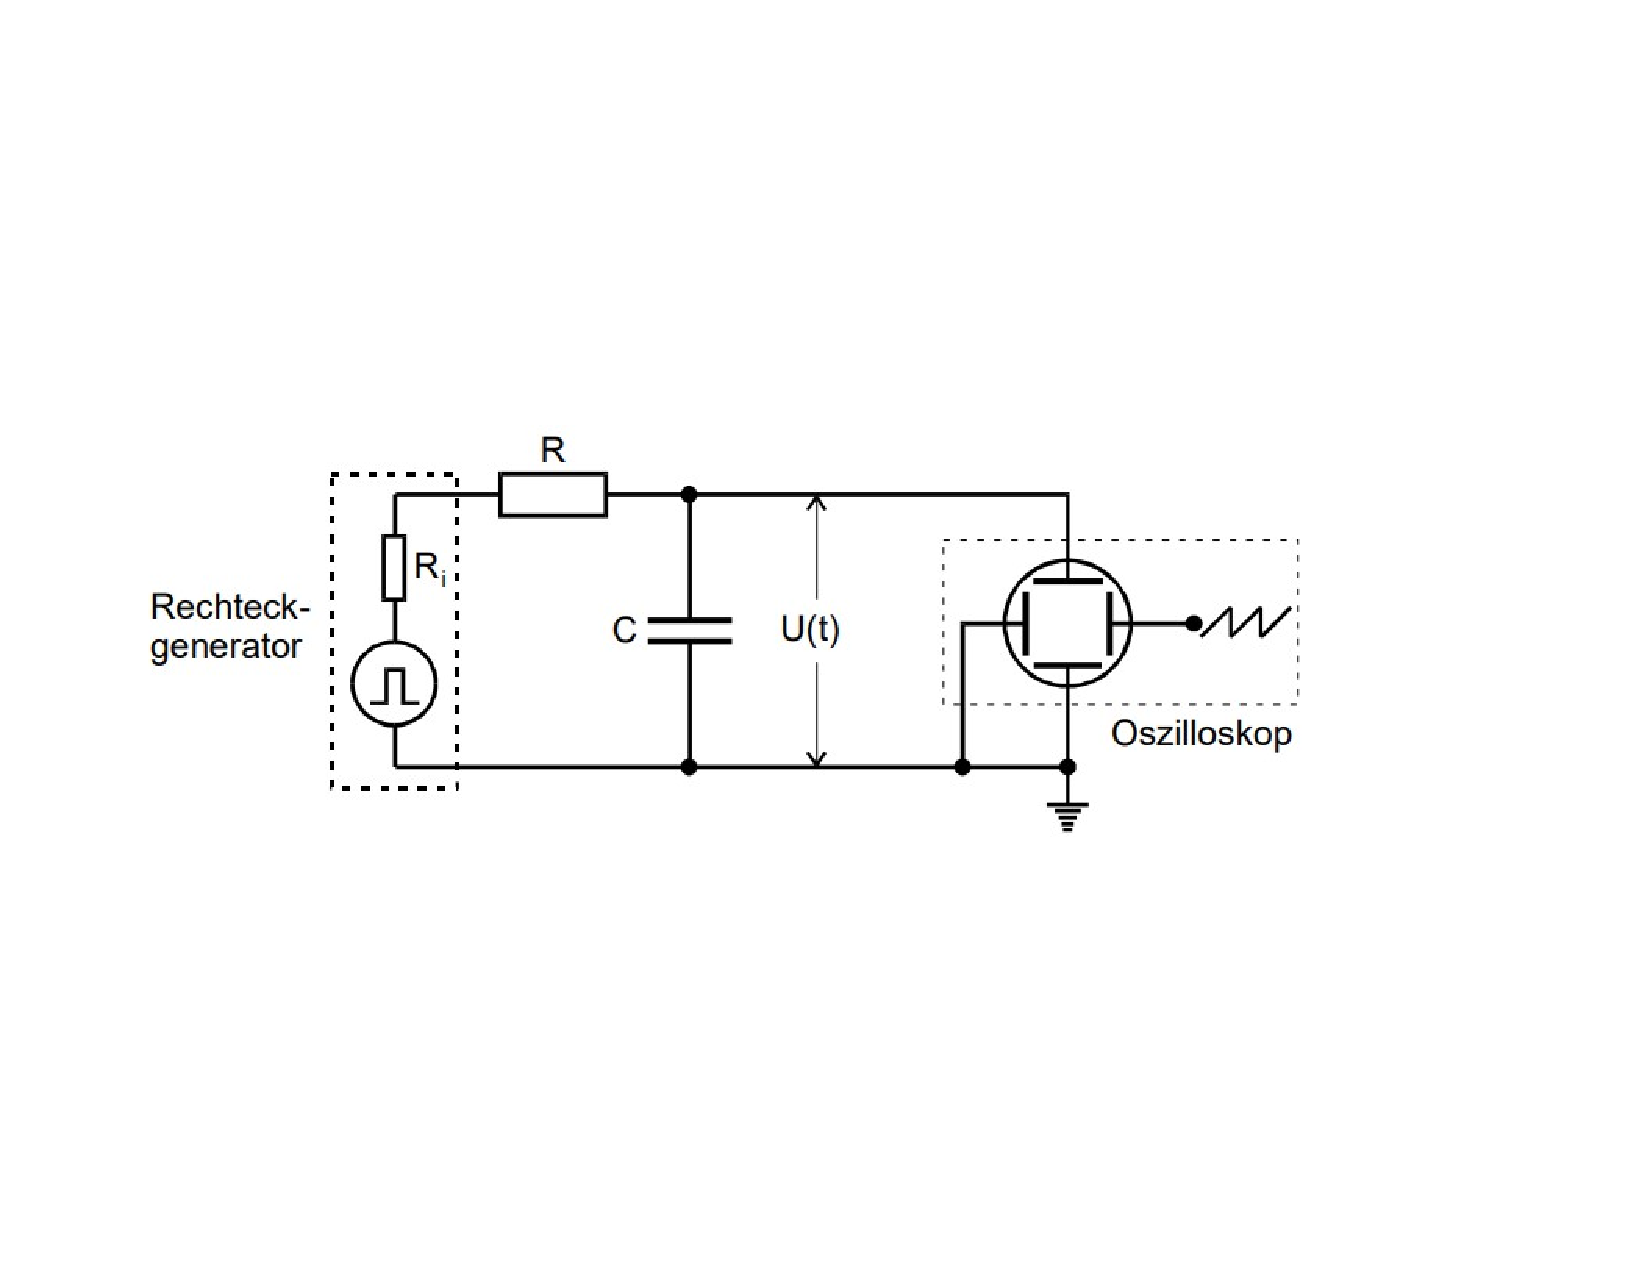
\includegraphics[width = 10cm]{V353foto4.pdf}
\caption{Aufbau für die erste Messreihe \cite{V353}}
\label{foto1}
\end{figure}

\begin{figure}
    \centering
    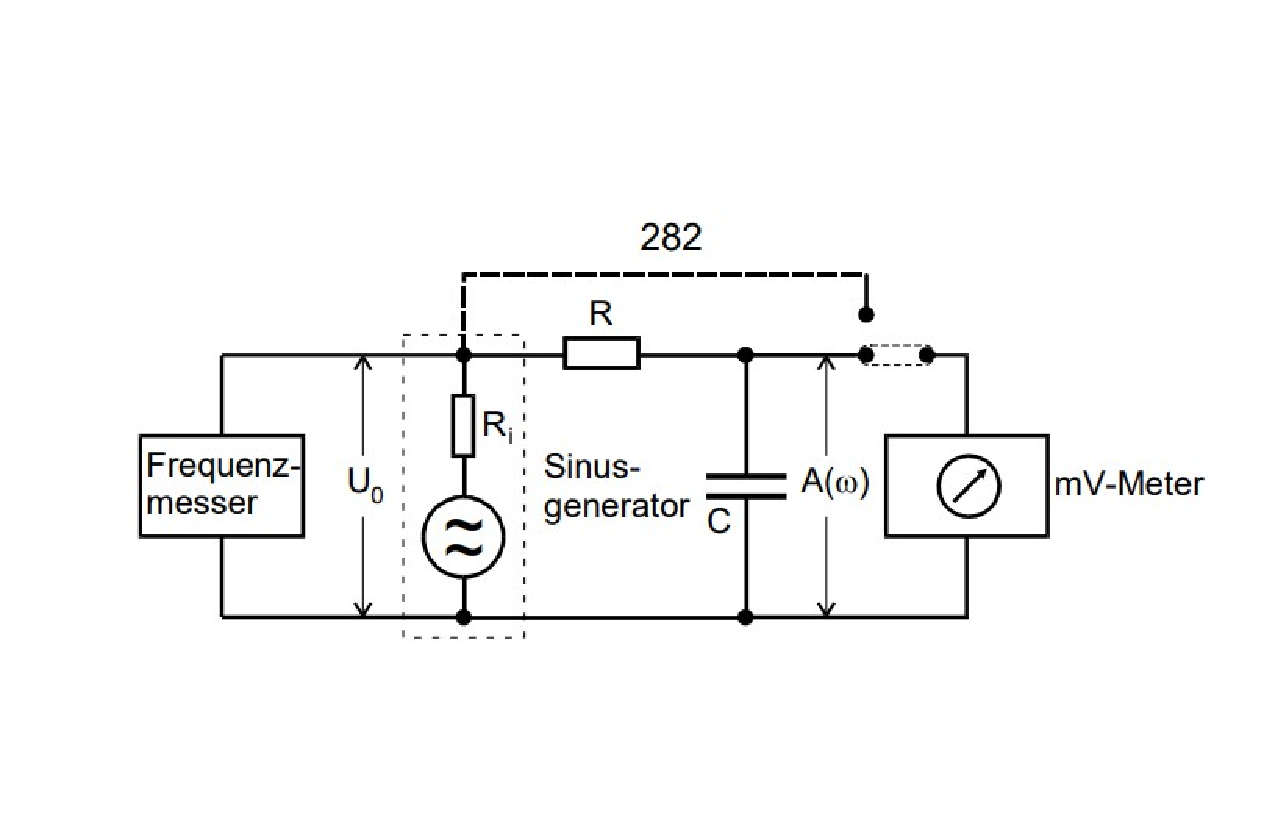
\includegraphics[width = 10cm]{V353foto5.pdf}
    \caption{Aufbau für die zweite Messreihe \cite{V353}}
    \label{foto2}
    \end{figure}

\subsection{Messreihe zur Entladekurve}
In der ersten messreihe werden Wertepaare der Spannung $U_c$ und der Zeit $t$ von der auf dem oszilloskop dargestellten Entladekurve abgelesen. 
Die Frequenz bleibt dabei konstant auf $77.2\unit{\hertz}$.
\subsection{Messreihe der Phasenverschiebung und der Spannungsamplitude}
In der zweiten Messreihe werden die Werte für die Phasenverschiebung zwischen der Generator- und der Kondensatorspannung und die Spannungsamplitude der Kondensatorspannung bei einer variierenden Frequenz $F$ 
von den auf dem oszilloskop dargestellten Kurven abgelesen. Die Messung wurde bei $F = 22000\unit{\hertz}$ aus technischen Gründen vorzeitig abgebrochen.
Gleichzeitig wird die Generatorspannungsamplitude abgelesen um zu versichern dass diese konstant bleibt.
\subsection{Messung zur Verifikation der Integratorfunktion}
Nun werden verschiedene Spannunsformen vom Spannungsgenerator erzeugt, die generierte Spannung wird gemeinsam mit der durch den Tiefpass integrierten Spannung auf dem Oszilloskop angezeigt,
die angezeigten Bilder werden Fotografiert. Es werden die Spannungen für eine Sinus- eine Dreieck- und eine Reckteckspannung fotografiert.


\section{Auswertung}
\label{sec:Auswertung}


In der nachfolgenden Tabelle \ref{tab:tabelle1} sind die gemessenen Werte der Stromstärke $I$ und des Abstandes $r$ sowie die aus $I$ nach \ref{} berechnete magnetische Flussdichte $B$ dargestellt.
Wobei $\mu_0 = 1.2566370621219 \cdot 10 ^ -6 $ gilt \cite{Formelsammlung}.
\begin{table}
  \centering
  \caption{Messwerte der Stromstärke, der magnetischen Flussdichte und des Abstandes r}
  \label{tab:tabelle1}
  \sisetup{table-format=1.1, per-mode=reciprocal}
  \begin{tblr}{
      colspec = {S[table-format=3.0] S[table-format=2.1] S},
      row{1} = {guard, mode=math},
    }
    \toprule
    r \mathbin{/} m \unit{\centimeter} [\pm 0.1mm]& I \mathbin{/} \unit{\ampere} [\pm 0.1 A] & B \mathbin{/} \unit{\tesla} [\pm 0.00014 T] & \\
    \midrule
    10.35 & 2.7  & 0.00366 \\
    9.95  & 2.6  & 0.00353 \\
    8.62  & 2.3  & 0.00312 \\
    8.29  & 2.0  & 0.00271 \\
    6.35  & 1.8  & 0.00244 \\
    5.78  & 1.6  & 0.00217 \\
    5.35  & 1.5  & 0.00203 \\
    4.9   & 1.4  & 0.00190 \\
    4.5   & 1.35 & 0.00183 \\
    4.05  & 1.3  & 0.00176 \\
    \bottomrule
  \end{tblr}
\end{table}

Um das magnetische Moment $\mu_{0}$ zu bestimmen wird nun mit polyfit \cite{numpy} eine lineare Regression aus den Messwerten erstellt. Zu sehen in Abbildung \ref{fig:plot1}.

\begin{figure}
  \centering
  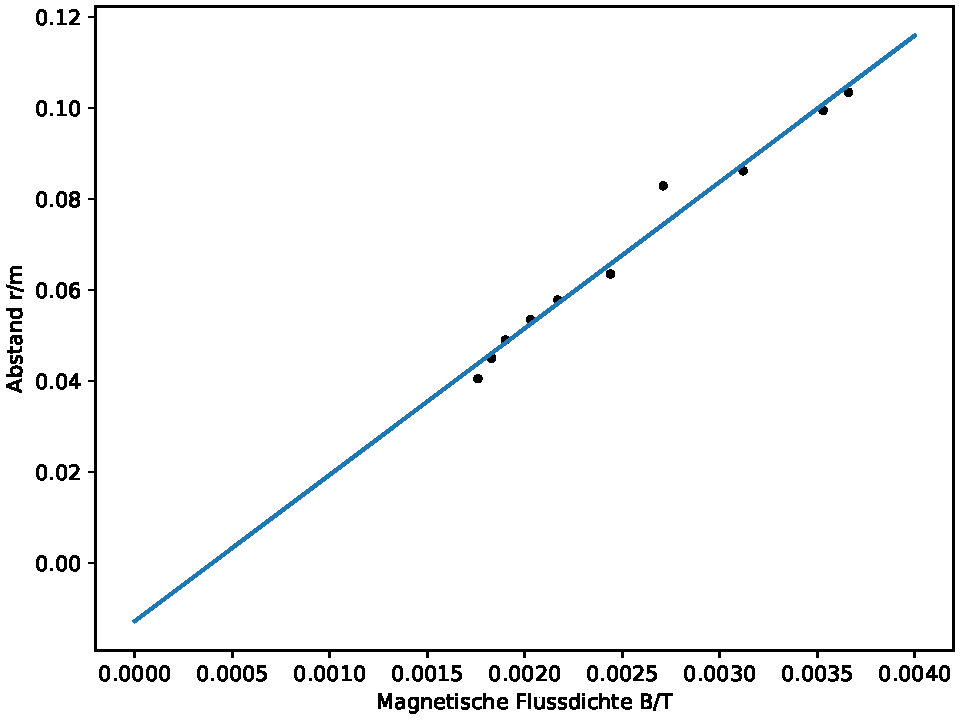
\includegraphics[width = 10cm]{plot1.pdf}
  \caption{Messwerte und lineare Regression von $r$ und $B$}
  \label{fig:plot1}
\end{figure}

Die ausgegebenen Parameter sind\\
\begin{centering}
  Steigung $a = (32.200 ± 1.639) \frac{m}{T}$\\
  Achsenabschnitt $b = (-0.013 ± 0.004)$m\\
\end{centering}

Nach \ref{} wird das magnetische moment aus der Steigung als\\
\begin{centering}
  $m \cdot g \cdot a = (0.442 \pm 0.023) Am^2$\\
\end{centering}
berechnet\\
Es wurde $g = 9.81$ verwendet. %EVENTUELLLLLLLLLLL QUEEEEEEEEELLLLLLLLLLLLLEEEEEEEEEEEEEEEE
\newpage
%----------------------------------------------------------------------- ZWEITE MESSUNG

In der folgenden Tabelle \ref{tab:tabelle2} werden die Messwerte für $I$, das daraus berechnete $B$ und die Periodendauer $T$ aufgeführt
\begin{table}
  \centering
  \caption{Messwerte der Stromstärke, der magnetischen Flussdichte und der Periodendauer T}
  \label{tab:tabelle2}
  \sisetup{table-format=1.1, per-mode=reciprocal}
  \begin{tblr}{
      colspec = {S[table-format=3.0] S[table-format=2.1] S},
      row{1} = {guard, mode=math},
    }
    \toprule
    I \mathbin{/} \unit{\ampere} [\pm 0.1 A] & B \mathbin{/} \unit{\tesla} [\pm 0.00014 T] & T \mathbin{/} \unit{\second} \\
    \midrule
    0.5  & 0.00068  & 3.154 \\
    0.7  & 0.00095  & 2.557 \\
    0.9  & 0.00122  & 2.006 \\
    1    & 0.00136  & 1.948 \\
    1.3  & 0.00176  & 1.625 \\
    1.5  & 0.00203  & 1.518 \\
    1.8  & 0.00244  & 1.380 \\
    2.3  & 0.00312  & 1.174 \\
    3    & 0.00407  & 1.047 \\
    3.5  & 0.00475  & 0.892 \\
    \bottomrule
  \end{tblr}
\end{table}

Zur Bestimmung des magnetischen Momentes wird nun in Abbildung \ref{fig:plot2} eine lineare Regression der Messwerte gemacht, dabei wird $T^2$ gegen $\frac{1}{B}$ aufgetragen.
\begin{figure}
  \centering
  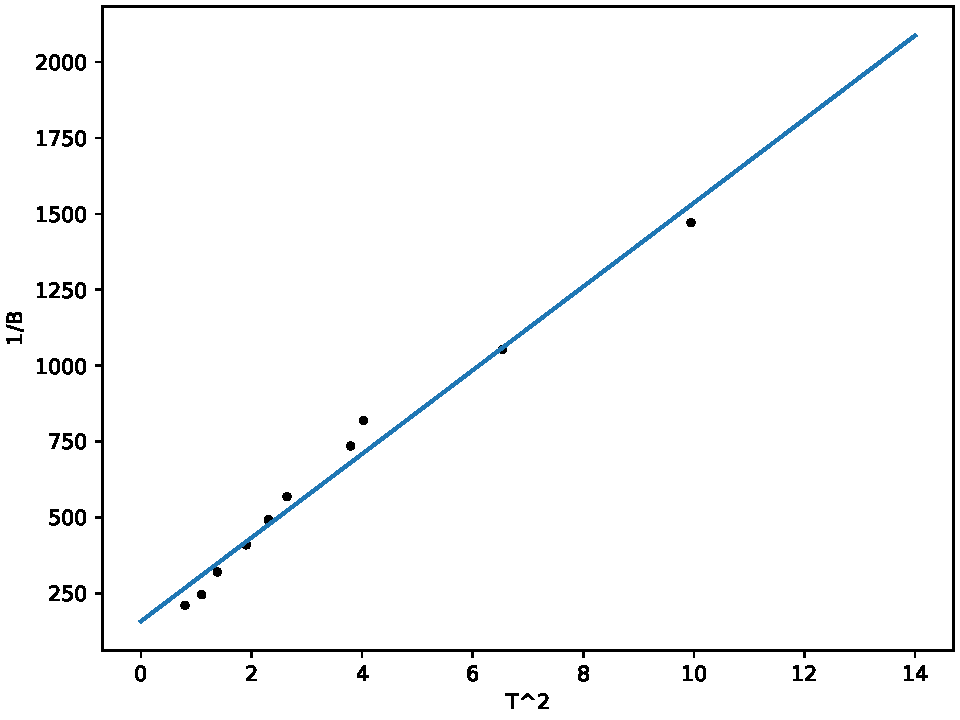
\includegraphics[width = 10cm]{plot2.pdf}
  \caption{Lineare Regression der Messwerte zur Bestimmung des magnetishen Momentes}
  \label{fig:plot2}
\end{figure}
Die von polyfit \cite{numpy} ausgegebenen Parameter sind\\

\begin{centering}
Steigung $a = (137.791 ± 6.958) s^2 \cdot T$\\
Achsenabschnitt $b = (158.221 ± 30.484) s^2$\\
\end{centering}

Das Trägheitsmoment der Billardkugel beträgt $Jk = \frac{2}{5}mr^2 = 4.704 \cdot 10^-5 kg\cdot m^2$\\

Nach \ref{} ergibt sich das magnetsiche Moment $\mu_0 = (0.256 \pm 0.013) Am^2$
\newpage

%______________________________________________________-- DRITTE MESSUNG

Für die dritte Methode der bestimmung des magnetischen Momentes in der folgenden Tabelle \ref{tab:tabelle3} die Messwerte für die Periodendauern, der Mittelwert der Periodendauern,
der Stromstärke $I$ und der daraus berechneten magnetischen Flussdichte $B$ aufgeführt.
\begin{table}
  \centering
  \caption{Messwerte der Stromstärke I, magnetische Flussdichte B, und 3 Präzessionsperioden Messwerte}
  \label{tab:tabelle3}
  \sisetup{table-format=1.1, per-mode=reciprocal}
  \begin{tblr}{
      colspec = {S[table-format=3.0] S[table-format=2.1] S},
      row{1} = {guard, mode=math},
    }
    \toprule
    I \mathbin{/} \unit{\ampere} [\pm 0.1 A] & B \mathbin{/} \unit{\tesla} [\pm 0.00014 T] & T_{\symup{p}1} \mathbin{/} \unit{\second} &   T_{\symup{p}2} \mathbin{/} \unit{\second} &  T_{\symup{p}3} \mathbin{/} \unit{\second} & \symup{Mittelwert der} T_p\\
    \midrule
    1    & 0.00136  & 15.77 & 15.35 & 15.9 & 15.67   \\
    1.5  & 0.00203  & 15.5  & 17.65 & 15.6 & 16.25   \\
    2    & 0.00271  & 13.0  & 11.63 & 11.61& 12.08   \\
    2.5  & 0.00339  & 9.7   & 9.44  & 9.59 & 9.58    \\
    3    & 0.00407  & 8.54  & 7.79  & 7.42 & 7.92    \\
  
    \bottomrule
  \end{tblr}
\end{table}

In der folgenden Abbildung \ref{fig:plot3} wird mithilfe von polyfit \cite{numpy} eine lineare regression der Messwerte erstellt.
\begin{figure}
  \centering
  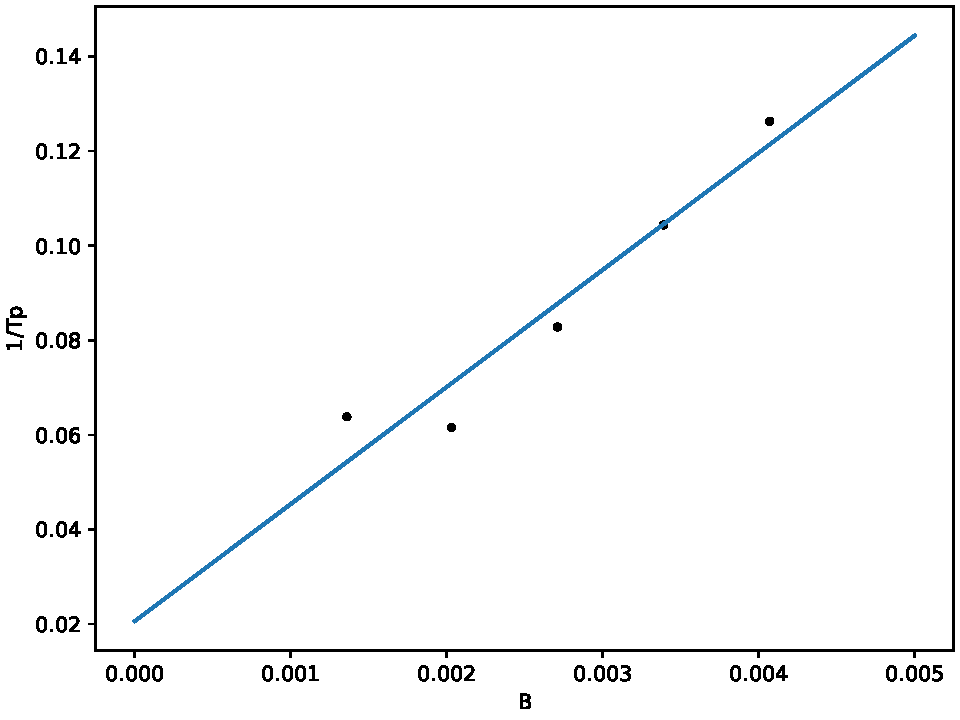
\includegraphics[width =10cm]{plot3.pdf}
  \caption{Lineare Regression zur Bestimmung des magnetischen momentes durch Präzession}
  \label{fig:plot3}
\end{figure}

Die ausgegebenen Parameter lauten\\
\begin{centering}
Steigung $a = (24.761 ± 4.049) \frac{1}{s \cdot T}$\\
Achsenabschnitt $b =(0.021 ± 0.012) \frac{1}{s}$\\
\end{centering}

Der Drehimpuls $L_{\symup{k}}$ berechnet sich nach \ref{} zu\\

\begin{centering}
  $L_{\symup{k}} = 1.241 \cdot 10^-3 N\cdot m\cdot s$
\end{centering}

Damit berechnet sich das magnetische Moment zu\\

\begin{centering}
  $\mu_0 = (0.193 \pm 0.032) Am^2$
\end{centering}
 



\section{Diskussion}
\label{sec:Diskussion}


\printbibliography{}

\section{Originale Werte}
\begin{figure}
\centering
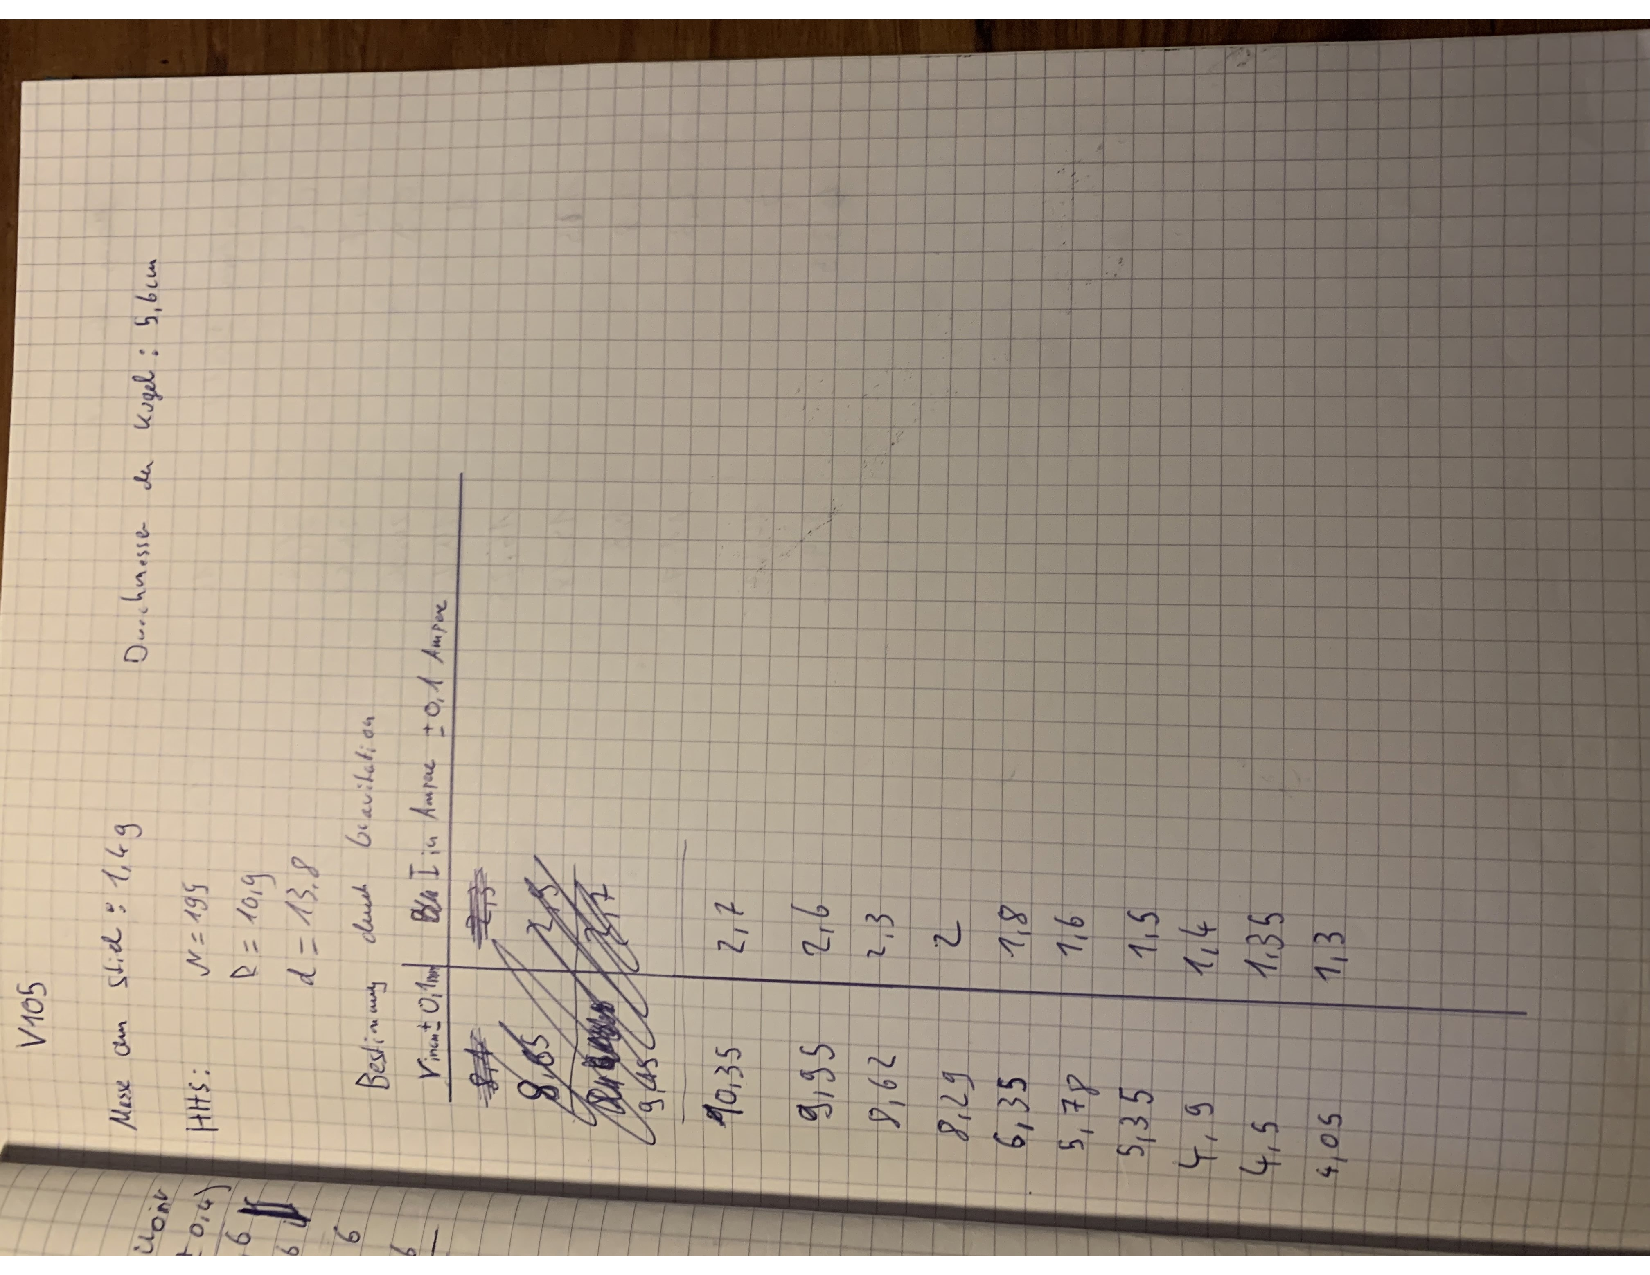
\includegraphics[width = 15cm]{V105foto1.pdf}
\caption{Originale Werte Seite 1}
\end{figure}
\begin{figure}
  \centering
  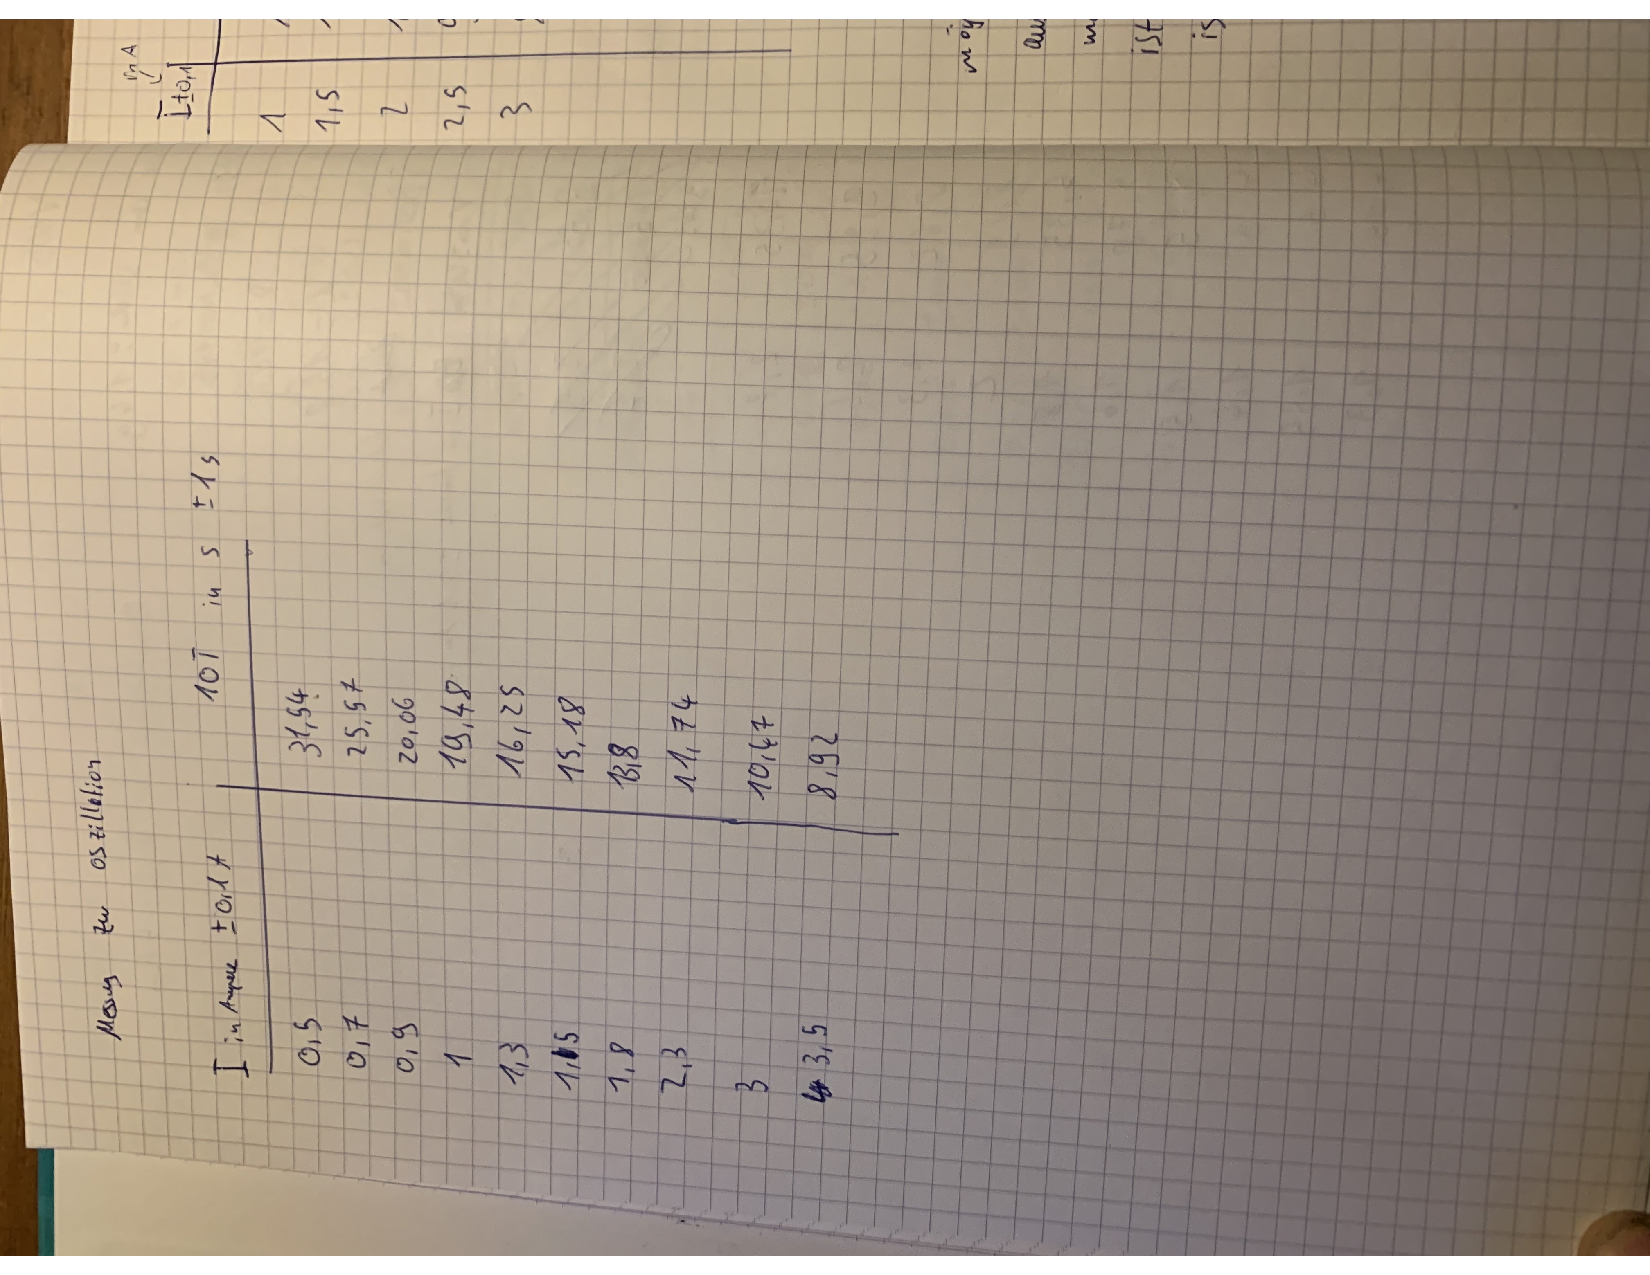
\includegraphics[width = 15cm]{V105foto2.pdf}
  \caption{Originale Werte Seite 2}
\end{figure}
\begin{figure}
  \centering
  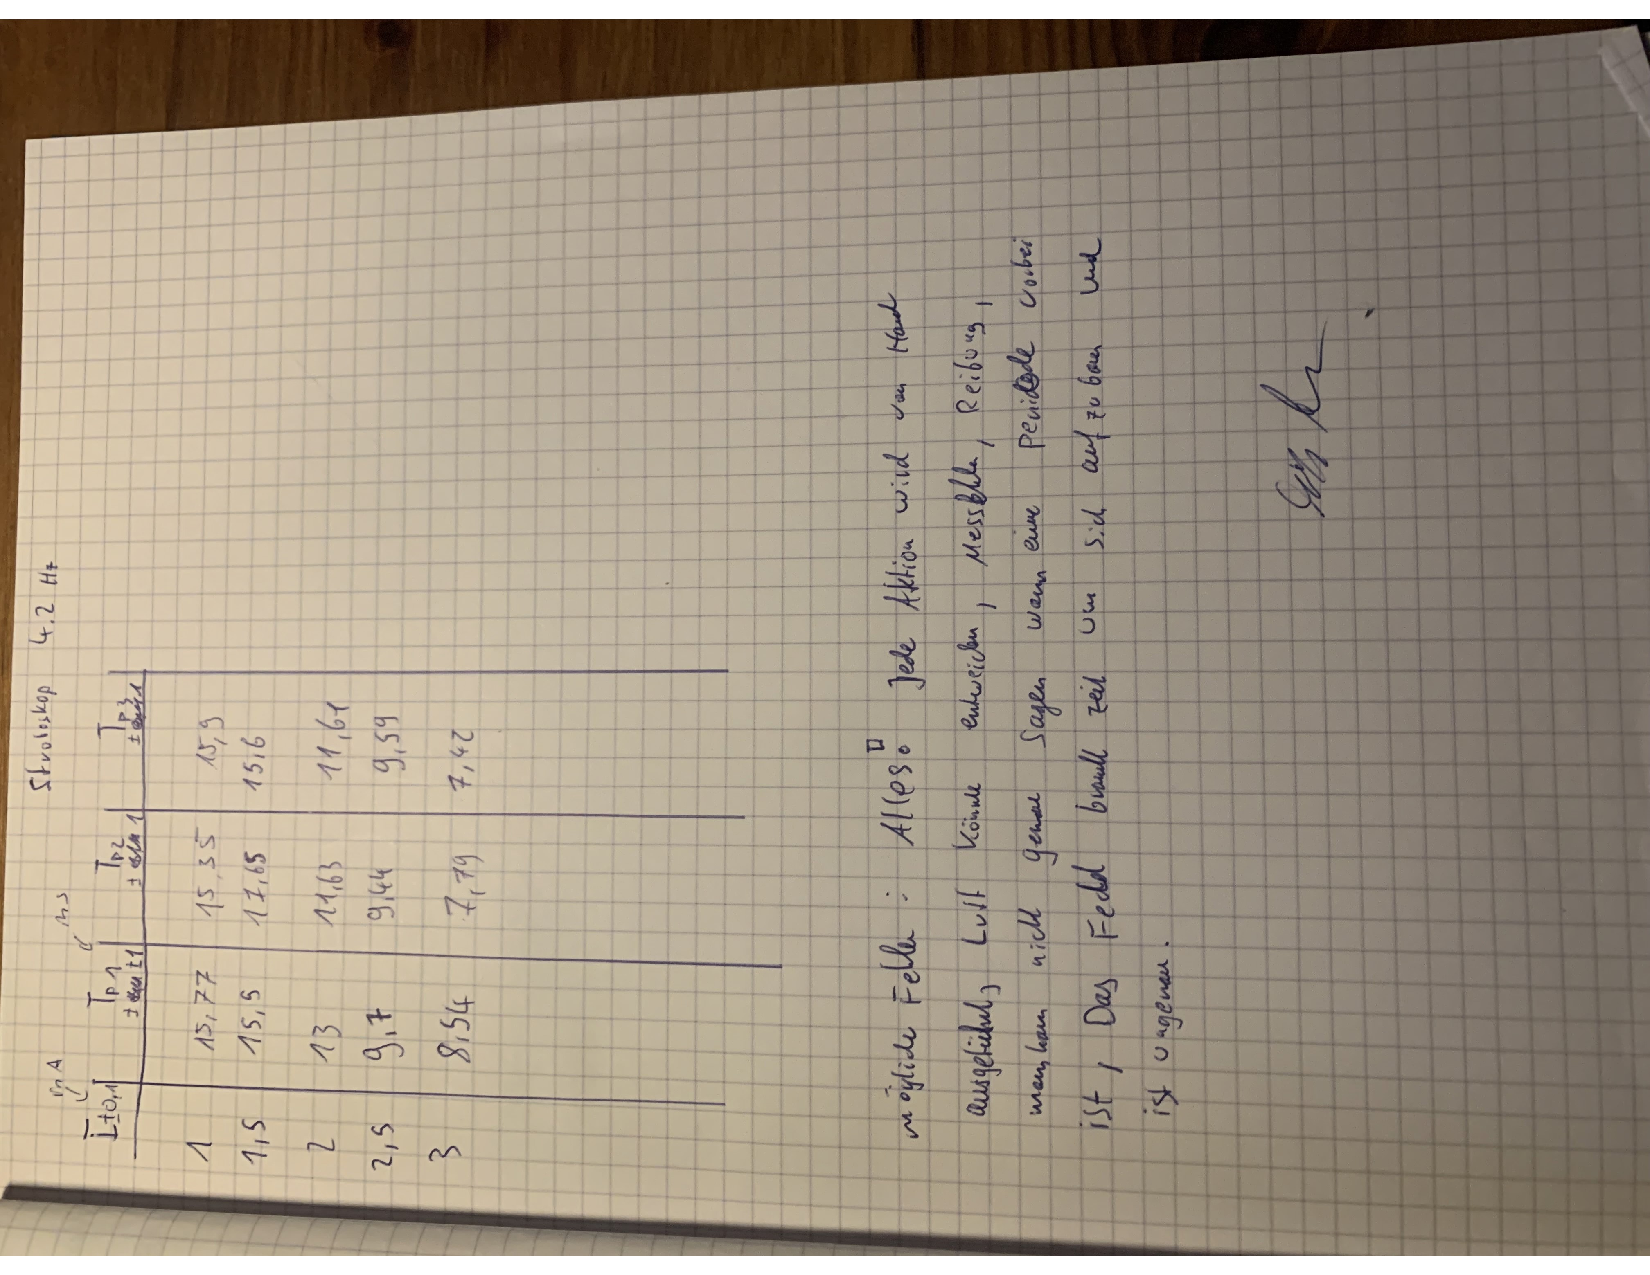
\includegraphics[width = 15cm]{V105foto3.pdf}
  \caption{Originale Werte Seite 3}
\end{figure}


\end{document}
